\chapter{Thiết kế hệ thống}
\label{chap:design}
\section{Thiết kế cơ sở dữ liệu}
\subsection{Lược đồ quan hệ và ERD}
Mô hình hiện hành được đối chiếu từ \texttt{\detokenize{store-admin/server/sql/schema.sql}} theo thứ tự migrations 001--017. Dump \texttt{\detokenize{database/schema.sql}} và \texttt{\detokenize{database/demo_data.sql}} là snapshot được tạo ngày 03/11/2026 sau migration 015, gồm 40 bảng; chúng không có bảng phiên đăng nhập mới ở migration 016--017. Sau hai migration này, schema hiện hành có thêm bảng \texttt{\detokenize{account_sessions}} với các trường IP và nguyên nhân thu hồi phiên. Hình~\ref{fig:erd} thể hiện các quan hệ nghiệp vụ chính; từ điển dữ liệu tại Phụ lục B mô tả thuộc tính của các bảng, gồm cả bảng phiên.
\IfFileExists{diagrams/04-erd.pdf}{\begin{figure}[htbp]\centering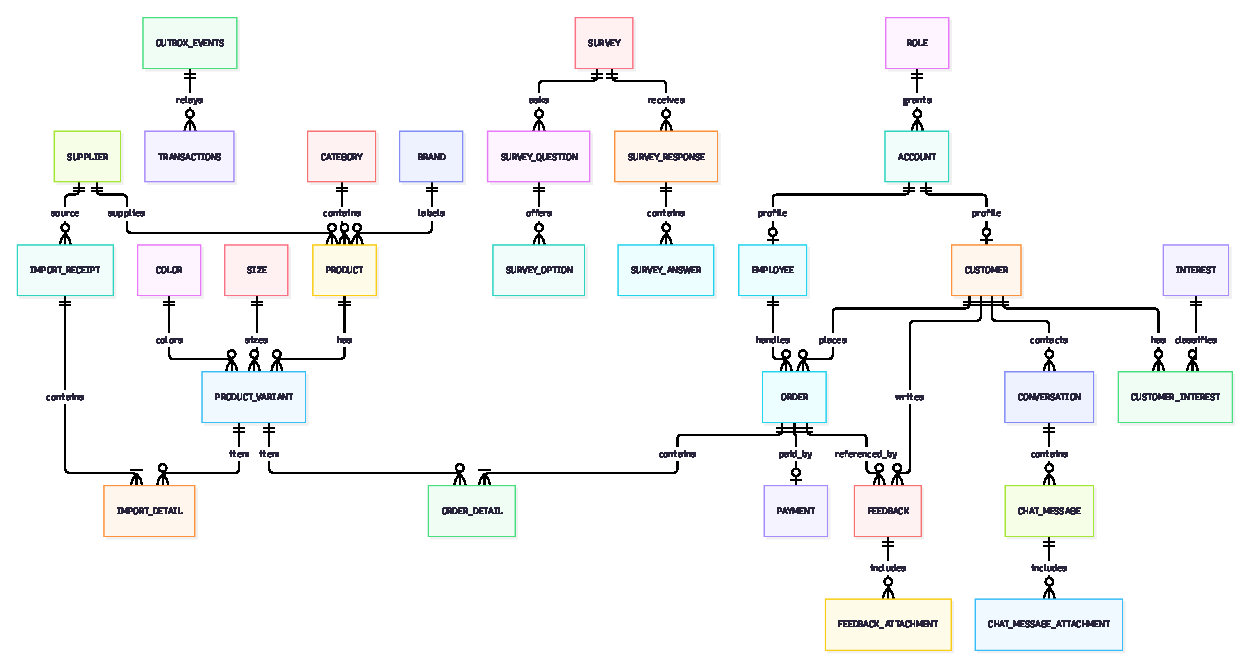
\includegraphics[width=\textwidth]{diagrams/04-erd.pdf}\caption{ERD các quan hệ nghiệp vụ chính theo SQL và migrations 001--017}\label{fig:erd}\end{figure}}{\begin{figure}[htbp]\centering\fbox{\parbox[c][2cm][c]{0.82\textwidth}{\centering [CHÈN ẢNH: ERD từ schema SQL hiện hành]}}\caption{ERD các quan hệ nghiệp vụ chính}\label{fig:erd}\end{figure}}

\subsection{Nguyên tắc thiết kế thể hiện trong DDL}
Các bảng nghiệp vụ dùng khóa chính số nguyên/identity hoặc UUID; quan hệ được khai báo bằng khóa ngoại; bảng nối như \texttt{\detokenize{role_permission}}, \texttt{\detokenize{customer_interest}}, \texttt{\detokenize{user_promotion}} có khóa ghép/unique chống liên kết trùng. Giá, số lượng, điểm đánh giá và miền trạng thái được giới hạn bằng CHECK/ENUM. \texttt{\detokenize{outbox_events.event_id}} và mã event mirror hỗ trợ nhận diện sự kiện; quan hệ Kafka/outbox là quan hệ xử lý ứng dụng, không phải khóa ngoại trực tiếp giữa hai bảng. Chi tiết từng trường, kiểu, khóa và index nằm ở Phụ lục B.

\subsection{Từ điển dữ liệu}
Từ điển Phụ lục B liệt kê các bảng từ snapshot 40 bảng cùng bảng \texttt{\detokenize{account_sessions}} được thêm ở migrations 016--017. Các thay đổi sau snapshot được mô tả theo file migration thay vì sửa dữ liệu dump mẫu. \texttt{\detokenize{customer_interest_map}} chỉ là bảng chuyển tiếp trong migration cũ; sau chuyển đổi, bảng nghiệp vụ là \texttt{\detokenize{customer_interest}}.

\section{Thiết kế giao diện}
Giao diện được triển khai bằng React. \texttt{\detokenize{client/src/App.jsx}} dùng một dashboard shell chung và tạo menu theo role; ADMIN có nhiều mục quản trị hơn, còn quản lý nhân sự/kho/bán hàng chỉ thấy các module được cấu hình cho role. Do đó, mã nguồn hiện chưa có một ứng dụng hoặc shell ADMIN riêng độc lập với các giao diện quản lý. Khách hàng dùng luồng đăng nhập và customer portal riêng. Các màn hình và điểm đặt ảnh minh chứng được liệt kê tại Bảng~\ref{tab:ui-screens}; thay ô ảnh bằng ảnh chụp thật đã che dữ liệu nhạy cảm.

\small
\begin{longtable}{|p{0.15\textwidth}|p{0.27\textwidth}|p{0.36\textwidth}|p{0.14\textwidth}|}
\caption{Các màn hình có trong mã nguồn và vị trí ảnh cần bổ sung}\label{tab:ui-screens}\\\hline
\textbf{Màn hình}&\textbf{Tệp giao diện chính}&\textbf{Chức năng/hoạt động và API}&\textbf{Ảnh minh chứng}\\\hline\endfirsthead
\multicolumn{4}{c}{Bảng~\ref{tab:ui-screens} (tiếp theo)}\\
\textbf{Màn hình}&\textbf{Tệp giao diện chính}&\textbf{Chức năng/hoạt động và API}&\textbf{Ảnh minh chứng}\\\hline\endhead
Đăng nhập nhân viên/quản trị&\texttt{\detokenize{AuthScreen.jsx}}&Đăng nhập tên đăng nhập/email; xác thực qua \texttt{\detokenize{POST /api/auth/login}}.&\fbox{[CHÈN ẢNH: Đăng nhập nhân viên]}\\\hline
Đăng nhập/đăng ký khách&\texttt{\detokenize{AuthScreen.jsx}}&Đăng ký hồ sơ, ngày sinh và sở thích; đăng nhập chỉ chấp nhận role khách tại \texttt{\detokenize{/api/auth/register}} và \texttt{\detokenize{/api/auth/login}}.&\fbox{[CHÈN ẢNH: Đăng nhập và đăng ký khách]}\\\hline
Catalog khách vãng lai&\texttt{\detokenize{CustomerPortal.jsx}}&Duyệt sản phẩm khi chưa đăng nhập; khách cần đăng nhập để đặt mua.&\fbox{[CHÈN ẢNH: Catalog khách vãng lai]}\\\hline
Tổng quan quản trị&\texttt{\detokenize{DashboardPage.jsx}}, \texttt{\detokenize{DashboardView.jsx}}, \texttt{\detokenize{AppShell.jsx}}&Hiển thị shell/menu và dữ liệu dashboard theo quyền.&\fbox{[CHÈN ẢNH: Tổng quan ADMIN]}\\\hline
Tài khoản và phân quyền&\texttt{\detokenize{AccountsView.jsx}}&Tìm tài khoản, tạo, đổi role, khóa/mở và xóa có điều kiện; \texttt{\detokenize{/api/accounts}}.&\fbox{[CHÈN ẢNH: Quản lý tài khoản]}\\\hline
Danh sách và bộ lọc sản phẩm&\texttt{\detokenize{ProductsView.jsx}}&Tìm tên/mô tả; lọc danh mục, thương hiệu, nhà cung cấp, giá; sắp xếp ngày tạo/tên/giá; CRUD và biến thể qua \texttt{\detokenize{/api/products}}.&\fbox{[CHÈN ẢNH: Sản phẩm và bộ lọc]}\\\hline
Tồn kho, phiếu kho, nhà cung cấp&\texttt{\detokenize{InventoryManagementView.jsx}}&Tra cứu tồn; lập phiếu nhập/xuất; nhập số lượng, giá nhập từng biến thể; tìm, lọc liên hệ, sắp xếp nhà cung cấp; \texttt{\detokenize{/api/inventory}}.&\fbox{[CHÈN ẢNH: Kho và nhà cung cấp]}\\\hline
Hồ sơ nhân viên&\texttt{\detokenize{EmployeesView.jsx}}&Tìm kiếm, thêm và cập nhật hồ sơ nhân viên qua \texttt{\detokenize{/api/employees}}.&\fbox{[CHÈN ẢNH: Nhân viên]}\\\hline
Đơn hàng&\texttt{\detokenize{OperationsView.jsx}}&Tra cứu/lọc đơn, tạo đơn tại quầy, xem chi tiết và thao tác trạng thái theo quyền; \texttt{\detokenize{/api/orders}}.&\fbox{[CHÈN ẢNH: Quản lý đơn hàng]}\\\hline
Khuyến mãi&\texttt{\detokenize{PromotionsView.jsx}}&Tạo, tìm và cập nhật chương trình theo loại/trạng thái; \texttt{\detokenize{/api/promotions}}.&\fbox{[CHÈN ẢNH: Khuyến mãi]}\\\hline
Quản lý khách hàng&\texttt{\detokenize{CustomersView.jsx}}&Tìm, xem hồ sơ, lịch sử và trạng thái khách; \texttt{\detokenize{/api/customers}}.&\fbox{[CHÈN ẢNH: Hồ sơ khách hàng CRM]}\\\hline
Phản hồi&\texttt{\detokenize{FeedbacksView.jsx}}&Tra cứu, đọc, trả lời và cập nhật trạng thái phản hồi; \texttt{\detokenize{/api/feedbacks}}.&\fbox{[CHÈN ẢNH: Xử lý phản hồi]}\\\hline
Khảo sát CRM&\texttt{\detokenize{SurveysView.jsx}}&Tạo/sửa câu hỏi, chọn đối tượng, gửi khảo sát, xem kết quả; \texttt{\detokenize{/api/surveys}}.&\fbox{[CHÈN ẢNH: Quản lý khảo sát]}\\\hline
Báo cáo&\texttt{\detokenize{ReportsView.jsx}}&Tab bán hàng, kho, nhân sự, khách hàng, phản hồi/khảo sát; lọc ngày và xuất CSV theo role; \texttt{\detokenize{/api/reports}}.&\fbox{[CHÈN ẢNH: Báo cáo theo vai trò]}\\\hline
Nhật ký và cài đặt&\texttt{\detokenize{AuditLogView.jsx}}, \texttt{\detokenize{SettingsView.jsx}}&Tra cứu nhật ký và cấu hình quản trị qua API tương ứng; cài đặt chỉ dành cho ADMIN.&\fbox{[CHÈN ẢNH: Nhật ký và cài đặt]}\\\hline
Chat CSKH cho nhân viên&\texttt{\detokenize{CustomerSupportChatView.jsx}}, \texttt{\detokenize{CskhChatView.jsx}}&Chọn hội thoại, gửi tin và xử lý trạng thái qua \texttt{\detokenize{/api/chat}}.&\fbox{[CHÈN ẢNH: Chat CSKH nhân viên]}\\\hline
Giỏ hàng và thanh toán&\texttt{\detokenize{CartView.jsx}}, \texttt{\detokenize{CheckoutView.jsx}}&Xem giỏ, địa chỉ giao hàng, phương thức thanh toán và trạng thái đơn; QR chỉ là DEMO.&\fbox{[CHÈN ẢNH: Giỏ hàng và thanh toán]}\\\hline
Đơn hàng của khách&\texttt{\detokenize{CustomerOrdersView.jsx}}&Xem danh sách/chi tiết và trạng thái các đơn của chính khách.&\fbox{[CHÈN ẢNH: Đơn hàng của khách]}\\\hline
Hồ sơ, điểm và voucher&\texttt{\detokenize{CustomerPortal.jsx}}, \texttt{\detokenize{CustomerLoyaltyView.jsx}}, \texttt{\detokenize{CustomerVouchersView.jsx}}&Cập nhật hồ sơ/sở thích, xem điểm và voucher của tài khoản.&\fbox{[CHÈN ẢNH: Hồ sơ, điểm thưởng và voucher]}\\\hline
Đánh giá và khảo sát của khách&\texttt{\detokenize{FeedbackMedia.jsx}}, \texttt{\detokenize{CustomerPortal.jsx}}&Gửi phản hồi, xem khảo sát được mời và gửi câu trả lời.&\fbox{[CHÈN ẢNH: Đánh giá và khảo sát]}\\\hline
Chat của khách&\texttt{\detokenize{StaffChatView.jsx}}, \texttt{\detokenize{CustomerPortal.jsx}}&Trao đổi trong hội thoại thuộc khách hàng; media chỉ xem theo quyền truy cập.&\fbox{[CHÈN ẢNH: Chat của khách]}\\\hline
\end{longtable}
\normalsize

\subsection{Giao diện ADMIN và các thao tác quản trị}
ADMIN sử dụng dashboard shell chung nhưng menu có thêm tài khoản, nhân viên, sản phẩm, tồn kho, đơn hàng, CRM, báo cáo, nhật ký và cài đặt. Giao diện độc lập hoàn toàn với shell của các role khác: \textbf{chưa cài đặt}; hiện tại là một ứng dụng React với menu và quyền truy cập thay đổi theo role. Bảng dưới ghi trạng thái theo đúng route và component đã kiểm tra.
\small
\begin{longtable}{|p{0.18\textwidth}|p{0.43\textwidth}|p{0.24\textwidth}|p{0.10\textwidth}|}
\caption{Đối chiếu các chức năng ADMIN với mã nguồn}\label{tab:admin-coverage}\\\hline
\textbf{Mục ADMIN}&\textbf{Chức năng đã kiểm tra}&\textbf{Vị trí code}&\textbf{Trạng thái}\\\hline\endfirsthead
\multicolumn{4}{c}{Bảng~\ref{tab:admin-coverage} (tiếp theo)}\\
\textbf{Mục ADMIN}&\textbf{Chức năng đã kiểm tra}&\textbf{Vị trí code}&\textbf{Trạng thái}\\\hline\endhead
Xem/tìm kiếm sản phẩm&Tìm tên/mô tả; lọc danh mục, thương hiệu, nhà cung cấp, khoảng giá; sắp xếp ngày mới, tên A--Z, giá tăng/giảm.&\texttt{\detokenize{ProductsView.jsx}}; \texttt{\detokenize{GET /api/products}}&Đã cài đặt\\\hline
Quản lý sản phẩm&Tạo/sửa/xóa sản phẩm, tạo biến thể size/màu/SKU và tồn ban đầu.&\texttt{\detokenize{ProductsView.jsx}}; \texttt{\detokenize{product.js}}&Đã cài đặt\\\hline
Xem/tìm nhà cung cấp&Tìm tên/người liên hệ/điện thoại/email; lọc có/thiếu email hoặc điện thoại; sắp xếp tên, người liên hệ, ngày tạo.&\texttt{\detokenize{InventoryManagementView.jsx}}; \texttt{\detokenize{inventory.js}} \texttt{\detokenize{GET /suppliers}}&Đã cài đặt\\\hline
Thêm/sửa nhà cung cấp&Thêm và cập nhật thông tin liên hệ, địa chỉ.&\texttt{\detokenize{InventoryManagementView.jsx}}; \texttt{\detokenize{POST/PATCH /api/inventory/suppliers}}&Đã cài đặt\\\hline
Xóa nhà cung cấp&Không có route DELETE nhà cung cấp trong \texttt{\detokenize{inventory.js}}.&--&Chưa cài đặt\\\hline
Tài khoản và quyền role&Tìm username/email; tạo tài khoản; đổi một trong các role có sẵn; khóa/mở; xóa nếu không phải tài khoản đang dùng, còn phiên, dữ liệu liên quan hay quản trị viên cuối cùng.&\texttt{\detokenize{AccountsView.jsx}}; \texttt{\detokenize{account.js}} \texttt{\detokenize{/api/accounts}}&Đã cài đặt\\\hline
Cấu hình quyền chi tiết&Không có giao diện CRUD ma trận \texttt{\detokenize{permission}}/\texttt{\detokenize{role_permission}}; chức năng hiện có đổi role theo danh mục.&\texttt{\detokenize{AccountsView.jsx}}; \texttt{\detokenize{account.js}}&Chưa cài đặt\\\hline
Giao diện ADMIN độc lập&Mã nguồn dùng shell chung, cấu hình menu theo role; không có ứng dụng/shell riêng chỉ cho ADMIN.&\texttt{\detokenize{App.jsx}}; \texttt{\detokenize{AppShell.jsx}}&Chưa cài đặt\\\hline
\end{longtable}
\normalsize

\subsection{Báo cáo kho và nhân sự}
Mục Báo cáo chỉ hiển thị tab theo role; API kiểm tra role ở backend. Quản lý kho (\texttt{QL\_KHO}) và ADMIN xem biến động nhập/xuất theo ngày trong khoảng chọn, giá trị tồn hiện tính bằng số lượng biến thể nhân giá nhập sản phẩm, biến thể có tồn không vượt ngưỡng và tổng nhập theo nhà cung cấp. Schema chưa có ngưỡng tồn tối thiểu riêng; màn hình nhận tham số, mặc định 10. Mỗi bảng có chức năng xuất CSV. Các API là \texttt{GET /api/reports/warehouse/movements}, \texttt{/warehouse/summary} và \texttt{/warehouse/suppliers}.

Quản lý nhân sự (\texttt{QL\_NHAN\_SU}) và ADMIN xem tổng hồ sơ, phân bố theo trạng thái hoạt động/chức vụ, số nhân viên mới theo tháng dựa trên \texttt{employee.hire\_date}; có thể xuất CSV. API \texttt{GET /api/reports/hr/summary} chỉ tổng hợp hồ sơ hiện có. Chấm công, tính lương và nghỉ phép chưa cài đặt; không suy diễn các nghiệp vụ đó từ hồ sơ nhân viên.

\subsection{Module nhóm chọn: CRM}
\label{subsec:crm-coverage}
Nhóm chọn CRM vì code có hồ sơ khách hàng, phản hồi, khảo sát, chat và báo cáo phân khúc. Bảng phân biệt vai trò quản lý CRM (\texttt{QL\_KHACH\_HANG}) với khách sử dụng portal (\texttt{KHACH\_HANG}); “Đã cài đặt” nghĩa là có view/route trong repository, không thay cho nghiệm thu nghiệp vụ thực tế.
\small
\begin{longtable}{|p{0.17\textwidth}|p{0.28\textwidth}|p{0.32\textwidth}|p{0.11\textwidth}|}
\caption{Đối chiếu module CRM theo vai trò và vị trí triển khai}\label{tab:crm-coverage}\\\hline
\textbf{Chức năng CRM}&\textbf{Quản lý CRM}&\textbf{Khách hàng}&\textbf{Trạng thái}\\\hline\endhead
Hồ sơ khách&Tìm/xem/cập nhật/trạng thái qua \texttt{\detokenize{CustomersView.jsx}}, \texttt{\detokenize{customer.js}} \texttt{\detokenize{/api/customers}}.&Xem/cập nhật hồ sơ và sở thích qua \texttt{\detokenize{AuthScreen.jsx}}, \texttt{\detokenize{PUT /api/auth/me}}.&Đã cài đặt\\\hline
Đăng ký/tài khoản&Quản trị tạo hồ sơ khách theo quyền; không tạo mật khẩu tại form khách CRM nếu không có luồng tài khoản.&Tự đăng ký qua \texttt{\detokenize{POST /api/auth/register}}; role được gán là \texttt{\detokenize{KHACH_HANG}}.&Đã cài đặt\\\hline
Phân khúc khách&Thống kê độ tuổi/sở thích/nhóm khách qua \texttt{\detokenize{ReportsView.jsx}}, \texttt{\detokenize{report.js}}.&Không xem dữ liệu tổng hợp khách khác.&Đã cài đặt\\\hline
Đánh giá/phản hồi&Tra cứu, trả lời, đổi trạng thái qua \texttt{\detokenize{FeedbacksView.jsx}}, \texttt{\detokenize{feedback.js}}.&Gửi đánh giá và tệp được hỗ trợ qua \texttt{\detokenize{CustomerPortal.jsx}}, \texttt{\detokenize{feedback.js}}.&Đã cài đặt\\\hline
Khảo sát&Soạn câu hỏi, chọn đối tượng, gửi và xem kết quả qua \texttt{\detokenize{SurveysView.jsx}}, \texttt{\detokenize{survey.js}}.&Xem khảo sát được mời và gửi câu trả lời qua \texttt{\detokenize{CustomerPortal.jsx}}, \texttt{\detokenize{survey.js}}.&Đã cài đặt\\\hline
Hỗ trợ trực tuyến&Quản lý hội thoại và gửi tin qua \texttt{\detokenize{CustomerSupportChatView.jsx}}, \texttt{\detokenize{chat.js}}.&Nhắn CSKH trong hội thoại của mình qua \texttt{\detokenize{CustomerPortal.jsx}}, \texttt{\detokenize{chat.js}}.&Đã cài đặt\\\hline
Đơn hàng và loyalty&Tra cứu thông tin khách/đơn theo quyền; không thay đổi lịch sử điểm tùy ý.&Tạo/theo dõi đơn, xem điểm và voucher qua \texttt{\detokenize{CustomerOrdersView.jsx}}, \texttt{\detokenize{CustomerLoyaltyView.jsx}}, \texttt{\detokenize{CustomerVouchersView.jsx}}.&Đã cài đặt\\\hline
Chiến dịch marketing tự động&Không có engine tự động hóa hành trình hoặc gửi chiến dịch email/SMS trong route hiện hành.&Không có màn hình cấu hình nhận tin/automation.&Chưa cài đặt\\\hline
Chấm công/lương/nghỉ phép CRM/HR&Không thuộc module CRM và không có route/chức năng tương ứng trong source.&Không áp dụng.&Chưa cài đặt\\\hline
\end{longtable}
\normalsize

\subsection{Nguyên tắc bảo vệ dữ liệu và giới hạn nghiệp vụ}
Khách chỉ truy cập dữ liệu gắn với tài khoản của mình trên các route khách; người dùng nội bộ bị chặn theo role ở middleware và handler. Xóa hồ sơ/tài khoản bị giới hạn nếu còn đơn, phản hồi, điểm, hội thoại hoặc dữ liệu liên quan; giao diện đề xuất khóa tài khoản khi xóa không an toàn. Chức năng chăm sóc khách chưa có automation chiến dịch hoặc gửi thư/SMS tự động. Hệ thống không có task, chấm công, tính lương hay nghỉ phép.
